
\section{Preliminaries and Problem Formulation}
\label{sec:preliminaries}
We consider multi-stage tasks whose valid executions are characterized by known stage-independent feasibility requirements and unknown stage-dependent constraints on task features. Let $\mathcal{X}\subseteq\mathbb{R}^{d_x}$ denote the state space, and let $\Phi=\{\phi_j:\mathcal{X}\rightarrow\mathbb{R}\}_{j=1}^{F}$ be a given task-dependent feature bank. For a state $x_t$, the full feature vector is $\phi(x_t)=[\phi_1(x_t),\dots,\phi_F(x_t)]^\top\in\mathbb{R}^{F}$. Before learning, each feature dimension is standardized over the demonstrated data.

A task consists of $K$ ordered stages. For a trajectory $\tau=\{x_t\}_{t=1}^{T}$, its cutpoints are denoted by $B=\{b_k\}_{k=0}^{K}$ and satisfy $1=b_0<b_1<\cdots<b_K=T+1$. The cutpoints induce the stage intervals $\mathcal{I}_k(B)=\{b_{k-1},\dots,b_k-1\}$ and the corresponding stage subgoals $g_k(B)=x_{b_k-1}$. When learning from demonstrations, the cutpoints and intermediate stage endpoints are unknown and may differ across trajectories.

The unknown stage-wise constraint model of a task is represented by a mode matrix $\Gamma=[\gamma_{k,j}]\in\{\varnothing,\mathrm{eq},\mathrm{lb},\mathrm{ub}\}^{K\times F}$. Here, $\gamma_{k,j}=\varnothing$ indicates that feature $j$ is unconstrained in stage $k$, while $\mathrm{eq}$, $\mathrm{lb}$, and $\mathrm{ub}$ denote an equality constraint, a lower-bound inequality, and an upper-bound inequality, respectively. The constraint family of each feature is not specified in advance; every stage-feature pair is evaluated under all four modes.

For every constrained stage-feature pair, $\eta_{k,j}\in\mathbb{R}$ denotes its scalar constraint parameter. It specifies the target feature value for an equality constraint and the boundary value for an inequality constraint. The collection of active parameters is denoted by $\mathcal{P}=\{\eta_{k,j}:\gamma_{k,j}\neq\varnothing\}$. The mode and parameter of each stage-feature pair induce the feasible set
\begin{equation}
\mathcal{C}_{k,j}
=
\begin{cases}
\mathcal{X},
& \gamma_{k,j}=\varnothing,\\
\{x\in\mathcal{X}:\phi_j(x)=\eta_{k,j}\},
& \gamma_{k,j}=\mathrm{eq},\\
\{x\in\mathcal{X}:\phi_j(x)\geq\eta_{k,j}\},
& \gamma_{k,j}=\mathrm{lb},\\
\{x\in\mathcal{X}:\phi_j(x)\leq\eta_{k,j}\},
& \gamma_{k,j}=\mathrm{ub}.
\end{cases}
\label{eq:stage_feature_feasible_set}
\end{equation}

Given the stage-wise constraint model $(\Gamma,\mathcal{P})$, a trajectory length $T$, a start state $x_{\mathrm{start}}$, and execution-specific ordered subgoals $\{g_k\}_{k=1}^{K}$, a valid task execution is defined as a solution to the following feasibility problem:
\begin{equation}
\begin{aligned}
\text{find}\quad
& \tau=\{x_t\}_{t=1}^{T},\quad B=\{b_k\}_{k=0}^{K} \\
\text{s.t.}\quad
& 1=b_0<b_1<\cdots<b_K=T+1,\\
& x_1=x_{\mathrm{start}},\\
& x_{b_k-1}=g_k,
\qquad k=1,\dots,K,\\
& \tau\in\mathcal{C}_{\mathrm{known}},\\
& x_t\in\bigcap_{j=1}^{F}\mathcal{C}_{k,j},
\qquad
t\in\mathcal{I}_k(B),\quad k=1,\dots,K.
\end{aligned}
\label{eq:stagewise_feasibility_problem}
\end{equation}
Here, $\mathcal{C}_{\mathrm{known}}$ contains known trajectory-level feasibility requirements, such as system dynamics and known kinematic limits.

We are given a set of feasible demonstrations $\mathcal{D}=\{\tau^{(i)}\}_{i=1}^{N}$, where $\tau^{(i)}=\{x_t^{(i)}\}_{t=1}^{T_i}$. The demonstrations may have different lengths, start states, subgoals, and latent cutpoints, but share the same number and ordering of stages and the same stage-wise constraint model $(\Gamma,\mathcal{P})$. Each demonstration is assumed to satisfy \eqref{eq:stagewise_feasibility_problem} under its true latent cutpoints.

\begin{definition}[Stage-wise constraint learning from demonstrations]
Given feasible demonstrations $\mathcal{D}$, the number of stages $K$, and the feature bank $\Phi$, stage-wise constraint learning aims to recover:
\begin{enumerate}
    \item the shared constraint mode matrix $\Gamma=[\gamma_{k,j}]$, which specifies the constraint mode of every stage-feature pair;
    \item the scalar constraint parameters $\mathcal{P}=\{\eta_{k,j}:\gamma_{k,j}\neq\varnothing\}$.
\end{enumerate}
The demonstration-specific cutpoints and their induced intermediate subgoals are also unknown and are jointly estimated during learning as auxiliary latent variables.
\end{definition}

\section{Method}
\label{sec:method}

\subsection{Overview}
The key idea of SWCL is to use a shared constraint model itself to explain and segment the demonstrations. Rather than representing a stage with a generic feature distribution, SWCL evaluates each stage-feature pair under four constraint-specific modes: inactive, equality-constrained, lower-bound constrained, and upper-bound constrained, and let the algorithm decides the best constraint mode for each stage. The cutpoints can adapt to each demonstration, while the constraint modes and their active targets or boundaries are shared across demonstrations.

More specifically, let $B^{(i)}$ denote the latent cutpoints of demonstration $i$, and let $\mathcal{I}_k^{(i)}$ be its interval assigned to stage $k$. The shared constraint model consists of the mode matrix $\Gamma=[\gamma_{k,j}]$ and the active target or boundary parameters $\mathcal{P}=\{\eta_{k,j}:\gamma_{k,j}\neq\varnothing\}$. We further let $\boldsymbol{\kappa}=\{\kappa_k\}_{k=1}^{K}$ denote the shared parameters of an auxiliary motion-progress model. At a conceptual level, SWCL jointly learns the stage-wise constraints and demonstration cutpoints by maximizing the posterior objective
\begin{equation}
p\!\left(\{B^{(i)}\}_{i=1}^{N},\Gamma,\mathcal{P},
\boldsymbol{\kappa}\mid\mathcal{D}\right)
\propto
p(\Gamma)\,
\mathcal{L}_{\mathrm{con}}
\mathcal{L}_{\mathrm{prog}},
\label{eq:swcl_posterior}
\end{equation}
where $p(\Gamma)$ is the constraint-mode prior, $\mathcal{L}_{\mathrm{con}}$ is the likelihood that measures how well the feature observations agree with the stage-wise constraint model, and $\mathcal{L}_{\mathrm{prog}}$ measures whether the motion within each stage advances toward its endpoint. Priors on the remaining variables are assumed to be uniform and are omitted. We use $\mathcal{L}$ for likelihoods over the complete dataset and $\ell$ for negative log-likelihoods of individual intervals or demonstrations.

SWCL approximately maximizes \eqref{eq:swcl_posterior} using an alternating hard expectation-maximization (EM) procedure. The hard E-step selects one set of cutpoints for each demonstration under the current shared model, while the M-step updates all shared constraint modes, constraint parameters, and progress parameters from the recovered stage intervals. Section~\ref{sec:constraint_observation_models} defines the constraint observation models, as well as $\mathcal{L}_{\mathrm{con}}$, and $p(\Gamma)$. Section~\ref{sec:directional_progress} defines $\mathcal{L}_{\mathrm{prog}}$. Section~\ref{sec:hard_em_inference} then describes initialization and the two alternating updates.

\subsection{Constraint Observation Models}
\label{sec:constraint_observation_models}

For a candidate stage interval, each feature is evaluated under a mode $m\in\mathcal{M}=\{\varnothing,\mathrm{eq},\mathrm{lb},\mathrm{ub}\}$. Every mode defines a proper density for the observed feature values. The inactive mode describes ordinary local variation, whereas the three active modes express a task-level target or boundary shared across demonstrations. Besides the shared constraint parameter, each density may contain local distribution parameters that account for variation across individual demonstrations. This subsection defines these densities and local parameters; all shared modes and constraint parameters are optimized in the M-step discussed in Section~\ref{sec:hard_em_inference}. Figure~\ref{fig:soft_half_t_example} illustrates the distributions of four constraint modes on an example feature distribution.

\subsubsection{Equality Mode}

An equality-constrained feature is expected to remain close to a common task-level target $\eta_{k,j}$. Its observation model is
\begin{equation}
p_{\mathrm{eq}}
\!\left(\phi\mid\eta_{k,j},\sigma_{k,j}^{(i)}\right)
=
\mathcal{N}
\!\left(\phi;\eta_{k,j},(\sigma_{k,j}^{(i)})^2\right),
\qquad
\sigma_{k,j}^{(i)}\leq\bar{\sigma}_{\mathrm{eq}},
\label{eq:equality_observation_model}
\end{equation}
where the target $\eta_{k,j}$ is shared across demonstrations, while $\sigma_{k,j}^{(i)}$ describes the local dispersion of demonstration $i$ around that target. For a fixed target and candidate interval, we use the Gaussian maximum-likelihood scale capped at a hyperparameter $\bar\sigma_{\mathrm{eq}}$. This upper bound specifies how tightly the observations must concentrate around a shared target for an equality interpretation to remain plausible. The shared target itself is optimized across demonstrations in the M-step.

\subsubsection{Inequality Modes}

We adopt the modeling assumption that, when a one-sided inequality is active and sufficiently expressed in the demonstrations, its feature values exhibit a boundary-anchored distribution: the observations remain primarily on the feasible side, while a non-negligible amount of probability mass occurs near the boundary. This pattern provides evidence for identifying both the activation and direction of the inequality. In contrast, if all demonstrations remain far inside the feasible region and never approach the true boundary, the inequality is generally not identifiable from feasible demonstrations alone~\cite{chou2020local}. In such cases, prior knowledge about its activation and direction can instead be encoded through the configurable mode probabilities introduced later.

Mathematically, for an active inequality with shared boundary $\eta_{k,j}$, we define the signed slack and model the slack with a half-Student-$t$ density. To accommodate observation noise and occasional small violations, we attach a soft exponential tail to the infeasible side.
\begin{equation}
y_m(\phi;\eta_{k,j})
=
\begin{cases}
\phi-\eta_{k,j}, & m=\mathrm{lb},\\
\eta_{k,j}-\phi, & m=\mathrm{ub}.
\end{cases}
\label{eq:inequality_signed_slack}
\end{equation}
\begin{equation}
p_m(\phi\mid\eta_{k,j},\sigma_{k,j}^{(i)})
=
\frac{1}{Z_{\nu,\alpha}}
\begin{cases}
\dfrac{2}{\sigma_{k,j}^{(i)}}
t_\nu\!\left(\dfrac{y_m}{\sigma_{k,j}^{(i)}}\right),
& y_m\geq0,\\[0.9em]
\dfrac{2}{\sigma_{k,j}^{(i)}}t_\nu(0)
\exp\!\left(\dfrac{y_m}{\alpha\sigma_{k,j}^{(i)}}\right),
& y_m<0,
\end{cases}
\label{eq:soft_half_t_density}
\end{equation}
where  $t_\nu$ is the standard Student-$t$ density, $\sigma_{k,j}^{(i)}$ is a local scale, $\alpha=0.1$ is a fixed parameter controlling the boundary softness, and $Z_{\nu,\alpha}=1+2\alpha t_\nu(0)$ is the normalizing constant. The local scale describes how widely the feasible observations spread away from the shared boundary; it is estimated separately for every demonstration--stage interval.

Ideally, $\sigma_{k,j}^{(i)}$ would be estimated by maximizing the interval likelihood for a fixed mode and boundary. Because this would require an additional numerical optimization for every candidate interval and boundary, we instead determine it by matching the 90-th percentile of the feasible slacks to that of the  half-Student-$t$ distribution.

\subsubsection{Inactive Mode}

When feature $j$ is inactive in stage $k$, its values need not concentrate around a task-level shared parameter. We use a local Gaussian with a relatively large scale as a neutral reference model:
\begin{equation}
p_{\varnothing}
\!\left(\phi\mid\mu_{k,j}^{(i)},\sigma_{k,j}^{(i)}\right)
=
\mathcal{N}
\!\left(\phi;\mu_{k,j}^{(i)},(\sigma_{k,j}^{(i)})^2\right),
\quad
\sigma_{k,j}^{(i)}\geq c_{\mathrm{bg}}\bar{\sigma}_{\mathrm{eq}},
\label{eq:inactive_observation_model}
\end{equation}
where $\mu_{k,j}^{(i)}$ and $\sigma_{k,j}^{(i)}$ are estimated separately for each demonstration--stage interval by minimizing its Gaussian negative log-likelihood subject to the scale lower bound. We use $c_{\mathrm{bg}}=3$, which prevents the locally centered inactive model from mimicking an equality constraint by shrinking its variance. Thus, inactive feature distributions may differ across demonstrations without inducing a shared task constraint.


\begin{figure}[t]
    \centering
    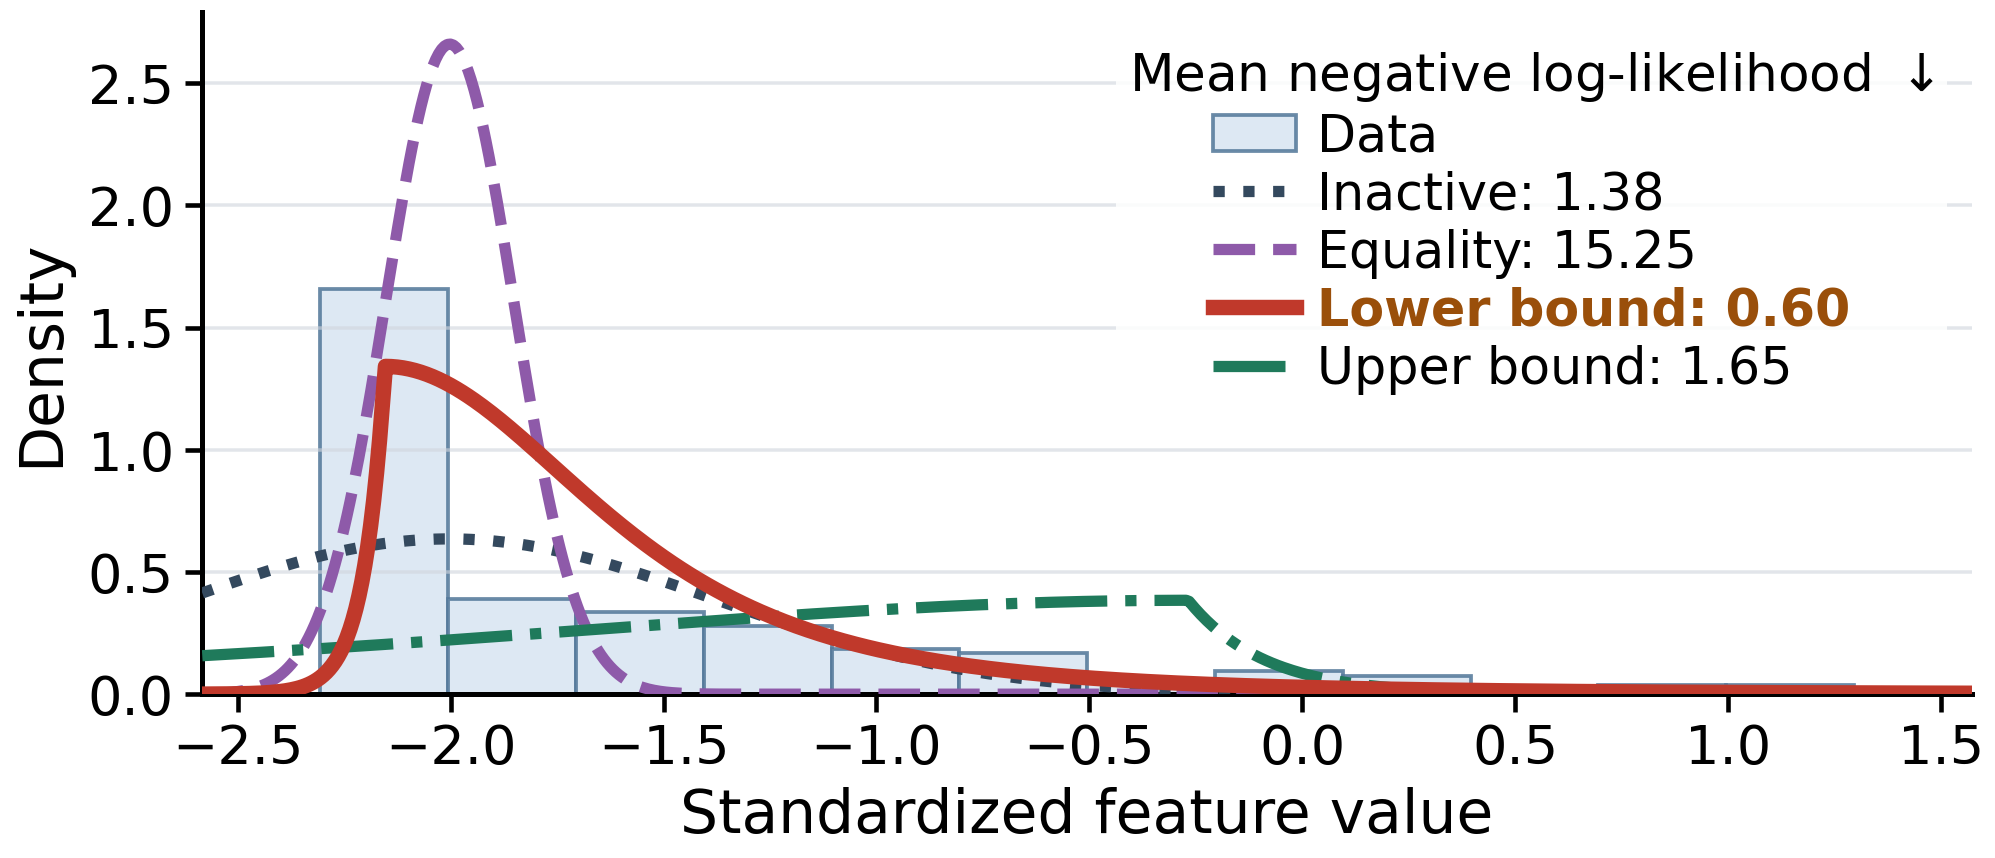
\includegraphics[width=0.85\linewidth]{figs/soft_half_t_example_distribution.png}
    \caption{Illustration of the four constraint-mode fits to an example dataset. Each curve uses its fitted parameters, and the legend reports the corresponding mean negative log-likelihood (lower is better). In this example, the lower-bound mode matches the data distribution the best and provides the strongest likelihood evidence.}
    \label{fig:soft_half_t_example}
\end{figure}


\subsubsection{Overall Constraint Likelihood and Mode Prior}
\label{sec:constraint_mode_prior}

For a candidate interval $\mathcal{I}$ from demonstration $i$ assigned to stage $k$, define the constraint negative log-likelihood
\begin{equation}
\ell_{\mathrm{con},k}^{(i)}(\mathcal{I})
=
\sum_{j=1}^{F}
\sum_{t\in\mathcal{I}}
-\log p_{\gamma_{k,j}}
\!\left(
\phi_j(x_t^{(i)})
\mid\eta_{k,j},\hat\psi_{k,j}^{(i)}(\mathcal{I})
\right),
\label{eq:interval_constraint_nll}
\end{equation}
where $\gamma_{k,j}\in\mathcal{M}$ is the single mode assigned to feature $j$ in stage $k$, and $p_{\gamma_{k,j}}$ denotes the corresponding density $p_{\varnothing}$, $p_{\mathrm{eq}}$, $p_{\mathrm{lb}}$, or $p_{\mathrm{ub}}$. The local parameters $\hat\psi_{k,j}^{(i)}(\mathcal{I})$ are fitted on the candidate interval using the rules above, while $\eta_{k,j}$ is omitted for the inactive mode. The complete likelihood $\mathcal{L}_{\mathrm{con}}$ in \eqref{eq:swcl_posterior} is obtained by multiplying the corresponding densities over all demonstration--stage intervals.

The likelihood alone may be insufficient to identify the correct mode, particularly when an inequality boundary is weakly expressed. SWCL therefore assigns each candidate a configurable prior probability $\pi_{k,j}(m)$, with
\begin{equation}
\pi_{k,j}(m)\geq0,
\qquad
\sum_{m\in\mathcal{M}}\pi_{k,j}(m)=1.
\label{eq:constraint_mode_prior}
\end{equation}
For example, if feature $j$ is known to be unconstrained in stage $k$, the prior probabilities of its equality, lower-bound, and upper-bound modes can all be set to zero. The full mode prior is $p(\Gamma)=\prod_{k=1}^{K}\prod_{j=1}^{F}\pi_{k,j}(\gamma_{k,j})$ and is applied once to each shared stage-feature mode.

\subsection{Directional Subgoal Progress}
\label{sec:directional_progress}

Relying solely on the constraint likelihood can lead to ambiguous segmentations and constraint interpretations. Recall from Section~\ref{sec:preliminaries} that we assume each stage is a goal-reaching task whose endpoint defines its subgoal. We therefore augment the objective with a subgoal-progress likelihood that characterizes whether the motion within a candidate stage consistently advances toward its endpoint.

A candidate interval $\mathcal{I}(s,e)=\{s,\ldots,e\}$ from demonstration $i$ induces the endpoint $g^{(i)}(\mathcal{I})=x_e^{(i)}$. For each nonzero transition inside the interval, we define the normalized directional-progress score
\begin{equation}
\delta_t^{(i)}(\mathcal{I})
=
\frac{
\|x_t^{(i)}-g^{(i)}(\mathcal{I})\|_2
-
\|x_{t+1}^{(i)}-g^{(i)}(\mathcal{I})\|_2
}
{\|x_{t+1}^{(i)}-x_t^{(i)}\|_2},
\label{eq:directional_progress}
\end{equation}
where $\delta_t^{(i)}\in[-1,1]$. A value near one indicates motion directly toward the endpoint, zero indicates approximately tangential motion, and a negative value indicates motion away from it. This term therefore favors candidate intervals in which the motion consistently approaches the endpoint. Motivated by von Mises--Fisher random-walk models, in which motion directions concentrate around a preferred direction~\cite{gatto2017saddlepoint}, we model the normalized progress score using the exponential-family density
\begin{equation}
p(\delta\mid\kappa_k)
=
\frac{\kappa_k\exp(\kappa_k\delta)}{2\sinh(\kappa_k)},
\qquad
\delta\in[-1,1],
\label{eq:progress_likelihood}
\end{equation}
with the limiting uniform density $p(\delta\mid0)=1/2$. For an interval containing $n$ valid transitions, its negative log-likelihood under stage $k$ is, up to the constant cost of the uniform reference density,
\begin{equation}
\ell_{\mathrm{prog},k}^{(i)}(\mathcal{I})
=
n\log\!\left(\frac{\sinh\kappa_k}{\kappa_k}\right)
-
\kappa_k
\sum_{t\in\mathcal{I}}
\delta_t^{(i)}(\mathcal{I}).
\label{eq:progress_interval_nll}
\end{equation}
The complete progress likelihood is the product of \eqref{eq:progress_likelihood} over all valid within-stage transitions in all demonstrations. Thus, $\kappa_k=0$ disables the progress contribution, whereas a larger $\kappa_k$ favors intervals that move consistently toward their endpoints. This term helps determine the stage cutpoints but is not interpreted as a learned task constraint.

\subsection{Hard-EM-like Inference}
\label{sec:hard_em_inference}

The cutpoints and shared model depend on each other: the model is estimated from the observations assigned to each stage, while the cutpoints are selected according to how well the resulting stages fit the current model. SWCL resolves this coupling by alternating the hard E-step and M-step described below.

\subsubsection{Hard E-step: Cutpoint Update}

With $(\Gamma,\mathcal{P},\boldsymbol{\kappa})$ fixed, the demonstrations can be processed independently. For a candidate interval $\mathcal{I}$ assigned to stage $k$, the constraint term is given by \eqref{eq:interval_constraint_nll}. Combining it with the progress term gives
\begin{equation}
\ell_k^{(i)}(\mathcal{I})
=
\ell_{\mathrm{con},k}^{(i)}(\mathcal{I})
+
\ell_{\mathrm{prog},k}^{(i)}(\mathcal{I}).
\label{eq:stage_interval_nll}
\end{equation}
The hard E-step selects
\begin{equation}
\hat B^{(i)}
=
\arg\min_{B^{(i)}}
\sum_{k=1}^{K}
\ell_k^{(i)}(\mathcal{I}_k^{(i)}).
\label{eq:hard_e_cutpoint_update}
\end{equation}
Because this objective is additive over consecutive stage intervals, it can be solved exactly for the current shared model by dynamic programming:
\begin{equation}
F_k^{(i)}(b_k)
=
\min_{b_{k-1}<b_k}
\left[
F_{k-1}^{(i)}(b_{k-1})
+
\ell_k^{(i)}(\mathcal{I}_k^{(i)})
\right],
\label{eq:dp_recurrence}
\end{equation}
where $\mathcal{I}_k^{(i)}$ is the candidate interval between $b_{k-1}$ and $b_k$, and $F_0^{(i)}(1)=0$. Backtracking from $F_K^{(i)}(T_i+1)$ recovers the complete cutpoint set $\hat B^{(i)}$. The update is hard because it retains this single MAP solution rather than a distribution over possible cutpoints.

\subsubsection{M-step: Shared-model Update}

With the cutpoints fixed, the observations assigned to every stage are known. The M-step jointly selects the shared mode and, when active, its shared target or boundary. For candidate mode $m$ and shared parameter $\eta$, define the demonstration-normalized negative log-likelihood
\begin{equation}
\ell_{k,j}^{(i)}(m,\eta)
=
\frac{1}{|\mathcal{I}_k^{(i)}|}
\sum_{t\in\mathcal{I}_k^{(i)}}
-\log p_m
\!\left(
\phi_j(x_t^{(i)})
\mid\eta,
\hat\psi_{k,j}^{(i)}(m,\eta)
\right),
\label{eq:demo_normalized_mode_nll}
\end{equation}
where the local parameters $\hat\psi_{k,j}^{(i)}(m,\eta)$ are fitted separately on each fixed demonstration--stage interval conditional on the candidate mode and shared parameter. The equality scale uses the capped Gaussian maximum-likelihood estimate, whereas the inequality scale uses the $90$th-percentile rule described above. Dividing by the interval length prevents demonstrations with longer stages or denser sampling from dominating the shared constraint estimate.

The shared mode and active parameter are updated by
\begin{equation}
(\hat\gamma_{k,j},\hat\eta_{k,j})
=
\arg\min_{m\in\mathcal{M},\,\eta}
\left[
\sum_{i=1}^{N}
\ell_{k,j}^{(i)}(m,\eta)
-\log\pi_{k,j}(m)
\right],
\label{eq:shared_mode_update}
\end{equation}
Operationally, SWCL evaluates the four modes separately. For each active mode, it first finds the target or boundary that minimizes the aggregated negative log-likelihood and retains the resulting mode-specific optimum. The inactive mode produces an analogous score without optimizing a shared parameter. SWCL then adds the corresponding negative log-prior to each optimized likelihood score and selects the mode with the smallest total; if an active mode is selected, its optimized target or boundary is retained as $\hat\eta_{k,j}$. The mode prior is applied once because $\gamma_{k,j}$ is one shared task-level variable. Since the lower- and upper-bound modes are separate candidates, this comparison determines both whether an inequality is active and its direction. The progress concentration of each stage is updated by

\begin{equation}
\hat\kappa_k
=
\arg\min_{\kappa\geq0}
\sum_{i=1}^{N}
\ell_{\mathrm{prog},k}^{(i)}
\!\left(\mathcal{I}_k^{(i)};\kappa\right).
\label{eq:progress_kappa_update}
\end{equation}

The E- and M-steps alternate until the cutpoints and shared model stabilize or a maximum number of iterations is reached.

\subsubsection{Initialization}
The first hard E-step requires an initial shared model. We begin by processing each demonstration independently. With $\boldsymbol{\kappa}=\mathbf{0}$, the progress density is uniform, and every candidate interval selects its best locally fitted constraint modes without sharing modes or constraint parameters across demonstrations. Dynamic programming then returns provisional cutpoints $B^{(i)}$. Treating the resulting intervals as corresponding stages, we perform the first M-step to initialize $(\Gamma,\mathcal{P},\boldsymbol{\kappa})$. Subsequent iterations use these shared parameters.

\begin{algorithm}[t]
\caption{Stage-Wise Constraint Learning}
\label{alg:swcl}
\begin{algorithmic}[1]
\Require demonstrations $\mathcal{D}$, number of stages $K$, feature bank $\Phi$, mode priors $\{\pi_{k,j}\}$
\Ensure cutpoints $\{\hat B^{(i)}\}$, constraint model $(\hat\Gamma,\hat{\mathcal{P}})$, progress parameters $\hat{\boldsymbol{\kappa}}$
\State Extract and standardize the feature trajectories
\ForAll{demonstrations $i=1,\ldots,N$}
    \State Initialize $B^{(i)}$ by locally fitting candidate intervals and applying dynamic programming
\EndFor
\State Initialize $(\Gamma,\mathcal{P},\boldsymbol{\kappa})$ from the provisional stage intervals
\Repeat
    \State \textbf{Hard E-step:}
    \ForAll{demonstrations $i=1,\ldots,N$}
        \State Update $B^{(i)}$ by \eqref{eq:dp_recurrence} and backtracking
    \EndFor
    \State \textbf{M-step:}
    \ForAll{stage--feature pairs $(k,j)$}
        \State Update $(\gamma_{k,j},\eta_{k,j})$ by \eqref{eq:shared_mode_update}
    \EndFor
    \ForAll{stages $k=1,\ldots,K$}
        \State Update $\kappa_k$ by \eqref{eq:progress_kappa_update}
    \EndFor
\Until{the cutpoints and shared model converge, or the maximum iteration is reached}
\State \Return $\{\hat B^{(i)}\}$, $\hat\Gamma$, $\hat{\mathcal{P}}$, and $\hat{\boldsymbol{\kappa}}$
\end{algorithmic}
\end{algorithm}
